\section{논의와 연구 범위}
\label{sec:discussion}

본 장에서는 5장의 결과가 무엇을 뜻하는지, 그리고 그 결과를 어디까지 해석할 수 있는지 설명한다. 핵심은 기본 CoC를 실행 가드로 보완하는 학습과, 실제 실행 단계에서 궤적을 다시 검사하는 일을 구분하는 것이다.

\subsection{기본 CoC와 실행 가드가 맡는 역할}

기본 CoC는 "보행자에게 양보한 뒤 진행한다"처럼 달성할 행동과 그 이유를 설명한다. 실행 가드는 "정지선을 넘지 않는다" 또는 "상충 구역이 1.5초 동안 비어 있을 때만 출발한다"처럼 그 행동을 언제, 어느 범위에서 허용할지를 정한다. Safety-Constrained CoC는 이 두 정보를 한 문맥에 넣은 CoC 통합형이다.

시간 조건 실험에서 요구사항 전용형의 가드 위반률은 0.319였지만 CoC 통합형은 0.000이었다. 이 결과는 기본 CoC가 위험하다는 뜻이 아니다. 기본 CoC에는 짧게 기다릴지 길게 기다릴지를 구분할 정보가 없었고, 실행 가드를 추가했을 때 모델이 그 차이를 배울 수 있었다는 뜻이다. 따라서 본 논문의 기여는 기존 CoC를 부정하는 것이 아니라, CoC가 말하지 않은 허용 조건을 학습 가능한 형태로 보완하는 데 있다.

\subsection{CoC 통합형이 높은 결과를 보인 이유}

시간 조건 실험에서 CoC 통합형은 가드를 분리해서 준 방식이나 논리식으로 준 방식보다 안정적인 결과를 보였다. 한 가지 가능한 이유는 기반 VLM이 자연어 문장에 익숙하고, CoC의 행동 목표와 실행 가드를 한 문맥에서 함께 처리할 수 있기 때문이다. 반대로 가드 분리형은 서로 떨어진 두 정보를 연결해야 하고, 논리식 가드는 모델이 익숙하지 않은 문법을 추가로 배워야 한다.

그러나 이 결과만으로 자연어가 논리식보다 본질적으로 우수하다고 결론 내릴 수는 없다. 정적 후보 실험에서는 논리식 가드도 위반률 0.000과 쌍 정확도 1.000을 기록하였다. 표현 방식을 공정하게 비교하려면 논리 문법을 따로 학습시키고, 각 조건에 같은 양의 학습 자료와 학습 횟수를 제공한 뒤 다시 평가해야 한다. 현재 결과가 직접 보여주는 것은 자연어의 보편적 우수성이 아니라, 현재 VLM과 학습 조건에서는 CoC 통합형이 가장 안정적이었다는 점이다.

\subsection{수치 조건은 독립 검증기가 다시 확인해야 한다}

어려운 표현 평가의 오답 15개는 모두 같은 거리를 m 대신 cm로 표현한 문장에서 발생하였다. 모델은 실행 가드의 일반적인 의미를 배웠지만, 수치와 단위를 바꾸는 계산까지 항상 정확하게 처리하지는 못했다. 따라서 실제 적용에서는 모델에 모든 계산을 맡기지 않고 그림~\ref{fig:future-architecture}과 같이 역할을 나누는 것이 적절하다.

먼저 모델은 자연어 Safety-Constrained CoC에서 행동 목표와 실행 가드의 의미를 읽는다. 다음 단계에서는 "최소 간격 600 cm"를 조건 종류, 비교 방향, 값과 단위로 나눈다. 그 뒤 600 cm를 6.0 m처럼 기준 단위로 통일한다. 마지막으로 독립 검증기 또는 차단장치가 선택한 궤적의 거리, 속도와 시간 조건을 수치로 검사한다.

이 과정에서는 "미만"과 "이하"처럼 경계값 포함 여부를 구분해야 한다. 또한 가드를 지킬 수 없을 때 정지할지, 다시 기다릴지와 같은 대체 행동도 정해야 한다. 모델은 문장의 목표와 조건을 해석하고, 검증기는 정확한 수치 경계를 확인하도록 역할을 나누는 것이다.

\begin{figure}[t]
\centering
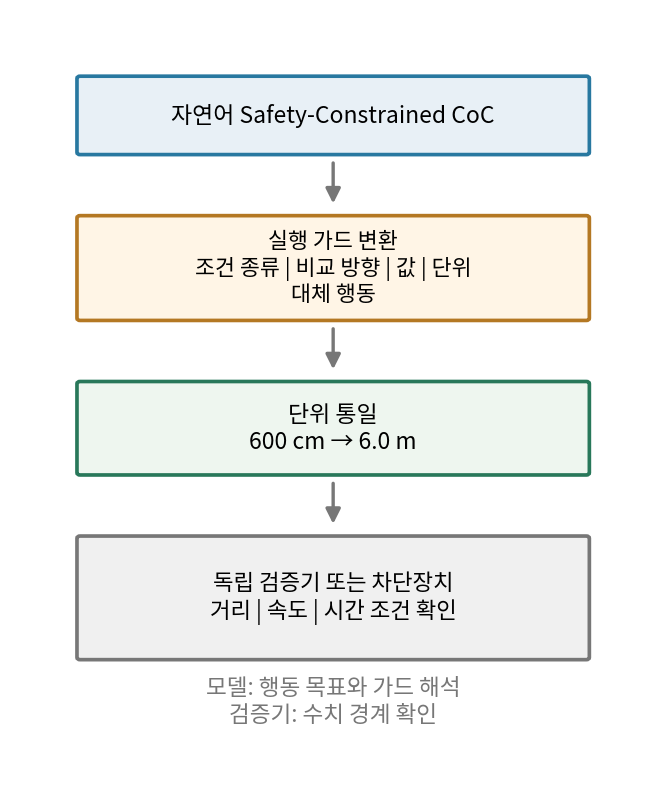
\includegraphics[width=0.94\columnwidth,trim=18 22 18 22,clip]{figures/fig05_typed_contract.png}
\caption{자연어 실행 가드를 실제 검사에 사용하는 네 단계. 모델은 행동 목표와 가드를 해석하고, 독립 검증기 또는 차단장치는 단위를 통일한 수치 조건을 확인한다.}
\label{fig:future-architecture}
\end{figure}

\subsection{학습된 가드와 실행 차단장치는 역할이 다르다}

가드를 학습하면 모델이 가드를 지키는 후보를 선택할 가능성이 높아진다. 그러나 학습에서 보지 못한 모든 상황에서 준수를 보장하지는 않는다. 폐루프의 해제 후 재위험 상황에서 동적 계약은 가드 위반률을 46.6\%에서 21.4\%로 줄였지만 위반을 없애지는 못했다. 최신 상태를 사용하는 차단장치를 함께 적용했을 때 위반률은 4.8\%까지 낮아졌다. 이는 학습된 계약과 실행 단계 검사가 서로 다른 역할을 맡는다는 것을 보여준다.

차단장치도 모든 문제를 해결하지는 못한다. 계약 정보가 0.4초 늦게 도착했을 때 계약+차단장치의 위반률은 34.8\%로 증가하였다. 계약 자체가 틀리거나 중요한 위험이 빠져 있어도 차단장치는 잘못된 조건을 정확하게 집행할 뿐이다. 따라서 실제 시스템에서는 위험이 다시 나타나면 출발 허용을 취소하고 대기 상태로 돌아갈 수 있어야 한다. 계약이 어느 시점의 상황을 설명하는지도 확인해야 하며, 미래 상황이 불확실하면 더 신중한 대체 행동을 선택해야 한다.

\subsection{주 실험이 실제로 확인한 것}

주 실험은 모델이 연속 궤적을 새로 생성하는 문제가 아니다. 합성 이미지와 수치가 적힌 궤적 후보를 주고 그중 하나를 선택하게 한 실험이다. 따라서 이 실험이 직접 확인한 것은 모델이 실행 가드를 읽고 후보 선택을 바꿀 수 있는가이다.

쌍대 계약은 같은 장면에서 가드만 바꾸므로 장면만 보고 같은 답을 반복하는 방법을 막는다. 가드 준수 목표 완료율은 모델이 가드 위반을 피하려고 끝까지 정지하는 방법도 막는다. 이 두 지표를 함께 사용하면 모델이 행동 목표를 끝내면서 가드에 맞는 후보를 골랐는지 확인할 수 있다. 그러나 후보의 물리량과 정답은 연구자가 설계했으며, 실제 차량의 복잡한 움직임이나 모든 충돌 위험을 포함하지 않는다. 그러므로 높은 점수는 제한된 후보 선택 문제에서의 가드 학습 효과이지 실제 차량 안전의 증명이 아니다.

\subsection{결과를 해석할 때의 실험적 한계}

후보 문자를 장면마다 바꾸어 같은 문자만 고르는 암기를 막았고, 대응을 섞은 가드로 문장 추가 자체의 효과를 구분하였다. 또한 학습의 무작위성을 바꾼 세 가지 초기값으로 실험을 반복하였다. 이러한 설계는 가드와 정답 후보의 관계를 실제로 학습했는지 확인하는 데 도움이 된다.

다만 반복 횟수가 세 번으로 적다. 어려운 표현 평가에는 단위 변환, 부정 표현, 경계값과 조건 순서 변경이 함께 들어 있다. 오답이 cm 문장에 집중되었지만, 현재 결과만으로 단위 변환 하나가 모든 오류의 원인이라고 확정할 수는 없다. 후속 실험에서는 장면과 나머지 문장을 고정하고 단위, 부정 표현, 경계값 포함 여부와 복합 조건을 한 번에 하나씩만 바꾸어 각 요인의 영향을 분리해야 한다.

\subsection{Alpamayo-R1과 실제 도로로 확장할 때의 범위}

작은 Qwen VLM의 후보 선택 결과가 Alpamayo-R1의 연속 궤적 생성에서도 그대로 나타난다고 볼 수는 없다. Alpamayo-R1 사전 진단은 모델이 CoC에 추가된 문장에는 반응하지만, 반대되는 가드의 의미를 안정적으로 구별하지 못했다는 결과만 제공한다. Alpamayo-R1에도 같은 효과가 있는지 확인하려면 가드 준수 학습을 직접 수행한 뒤 연속 궤적을 독립 검증해야 한다.

또한 본 논문의 실행 가드는 도로 안전 전체가 아니라 정지선, 최소 간격, 속도와 대기시간 같은 일부 조건만 다룬다. 실제 도로에서는 센서에 보행자나 차량이 실제로 보이는지, 보행자·자전거·차량의 위치와 이동 경로가 어떻게 겹치는지, 선택한 궤적의 충돌 위험은 얼마인지도 확인해야 한다. 계약이 센서의 어느 시점과 대응하는지 기록하고, 사람의 검토나 측정값으로 만든 독립된 정답 자료와 비교하는 평가도 필요하다. 따라서 다음 단계는 작은 VLM 결과를 실제 안전으로 확대 해석하는 것이 아니라, Alpamayo-R1의 연속 궤적과 실제 센서 근거에서 같은 질문을 다시 검증하는 것이다.
